\section{Methodology} \label{Method}



% \subsection{Problem Statement}\label{sec:problem}
% We represent each molecule as an Atoms-in-SMILES (AIS) \citep{article} token sequence ${\mathcal{G}}=\{m_1,\dots,m_K\}$, which provides a chemistry-aware, graph-informed alternative to character-level SMILES. For molecule captioning (G2S), we describe the structure by serializing the molecular graph into an edge-list sequence (denoted by $\tilde{\mathcal{G}}$), using special tokens \texttt{[HEAD]}, \texttt{[REL]}, \texttt{[TAIL]}, \texttt{[SEP]}:
% \[
% \resizebox{0.95\columnwidth}{!}{$
% \tilde{\mathcal{G}}=
% \big\langle
% \texttt{[HEAD]}\ h_i\ \texttt{[REL]}\ r_{ij}\ \texttt{[TAIL]}\ t_j\ \texttt{[SEP]}
% \big\rangle_{(i,j)}$}
% \]

% \noindent where $(h_i,r_{ij},t_j)$ denotes an atom-bond-atom triple.
% Let $\mathbf{S}_{\text{text}}=\{s_1,\ldots,s_N\}$ be a textual description. We study two conditional generation tasks:
% (i) \textbf{captioning} $\tilde{\mathcal{G}}\!\rightarrow\!\mathbf{S}_{\text{text}}$, and
% (ii) \textbf{molecule generation} $\mathbf{S}_{\text{text}}\!\rightarrow\!\tilde{\mathcal{G}}$.
% Accordingly, we learn $\mathcal{M}_\theta:\tilde{\mathcal{G}}\rightarrow \mathbf{S}_{\text{text}}$ and $\mathcal{M}_\phi:\mathbf{S}_{\text{text}}\rightarrow \tilde{\mathcal{G}}$ and maximize
% \[
% \max_{\Theta}\ \log p(\mathbf{S}_{\text{text}}\mid \tilde{\mathcal{G}};\theta)\ +\ \log p(\tilde{\mathcal{G}}\mid \mathbf{S}_{\text{text}};\phi),
% \]
% \vspace{-2mm}
% \noindent where $\Theta=\{\theta,\phi\}$. For evaluation, the generated $\tilde{\mathcal{G}}$ is deterministically mapped to a canonical SMILES string.







\subsection{Problem Statement}\label{sec:problem}
We use canonical SMILES as the standard molecule representation throughout
\texttt{BiMol-Diff}. From this canonical string view, we derive two related
representations. First, we denote by
$G = \{m_1,\ldots,m_K\}$ the Atoms-in-SMILES (AIS)~\citep{article} token sequence,
which provides a chemistry-aware alternative to character-level SMILES.
Second, for graph-conditioned modeling, we denote by $\tilde{G}$ the
serialized molecular graph obtained by writing the molecule as an
edge-list sequence of atom--bond--atom triplets using special tokens
\texttt{[HEAD]}, \texttt{[REL]}, \texttt{[TAIL]}, and \texttt{[SEP]}:
\[
\tilde{G}
=
\big\langle
\texttt{[HEAD]}~h_i~
\texttt{[REL]}~r_{ij}~
\texttt{[TAIL]}~t_j~
\texttt{[SEP]}
\big\rangle_{(i,j)},
\]
where $(h_i,r_{ij},t_j)$ denotes an atom-bond-atom triple.
Let $S_{\text{text}} = \{s_1,\ldots,s_N\}$ be a textual description.
We study two conditional generation tasks:
(i) \textbf{molecule captioning} $\tilde{G} \rightarrow S_{\text{text}}$, and
(ii) \textbf{molecule generation} $S_{\text{text}} \rightarrow \tilde{G}$.
Accordingly, we learn
$M_\theta : \tilde{G} \rightarrow S_{\text{text}}$ and
$M_\phi : S_{\text{text}} \rightarrow \tilde{G}$ and maximize
\[
\max_{\Theta}
\log p(S_{\text{text}} \mid \tilde{G}; \theta)
+
\log p(\tilde{G} \mid S_{\text{text}}; \phi),
\]
where $\Theta=\{\theta,\phi\}$.
We next describe the molecule-side representation pipeline used to realize these two directions, starting from canonical SMILES and proceeding through AIS-aware tokens and serialized graph sequences.




\subsection{The \texttt{BiMol-Diff} Framework Overview}

We introduce \texttt{BiMol-Diff}, a unified diffusion framework that addresses
molecular graph-to-sequence (G2S) and sequence-to-graph (S2G)
generation under a single conditional modeling view. Given paired data \((\mathcal{A}, \mathcal{B}) \in \{(\mathbf{S_{text}}, \tilde{\mathcal{G}}), (\tilde{\mathcal{G}}, \mathbf{S_{text}})\}\), \texttt{BiMol-Diff} learns the conditional distribution \(p(\mathcal{A}\mid \mathcal{B})\), where \(\mathcal{B}\) provides the conditioning context and \(\mathcal{A}\) is the target modality.

% \noindent \textbf{Graph Encoding.}
% We represent a molecule as triplets \(\tilde{\mathcal{G}}=\{(h_i,r_{ij},t_j)\}\) and serialize them into a single token sequence (with \texttt{[HEAD]/[REL]/[TAIL]} templates and \texttt{[SEP]} delimiters) to condition a transformer backbone in the G2S direction (Section~\ref{sec:graph-encoding}); conversely, \(\mathbf{S_{text}}\) conditions reconstruction of \(\tilde{\mathcal{G}}\) in S2G.

\noindent \textbf{Molecule Representation Pipeline.}
We use canonical SMILES as the common molecule interface in both directions and convert it to its Atoms-in-SMILES representation \(G\)~\citep{article}. For graph-conditioned modeling, this molecule-side representation is deterministically mapped to the serialized graph sequence \(\tilde{G}\), where each bond is written as an atom-bond-atom triplet using \texttt{[HEAD]/[REL]/[TAIL]} templates and \texttt{[SEP]} delimiters. Thus, in the G2S direction, \(\tilde{G}\) serves as the conditioning sequence for generating \(\mathbf{S_{text}}\). Conversely, in the S2G direction, \(\mathbf{S_{text}}\) conditions prediction of \(\tilde{G}\), and the predicted \(\tilde{G}\) is deterministically mapped back through the same molecule-side representation pipeline into canonical SMILES for evaluation. Figure~\ref{fig:enc_dec} summarizes this symmetric encoding/decoding view.

\begin{figure}[h!]
    \centering
    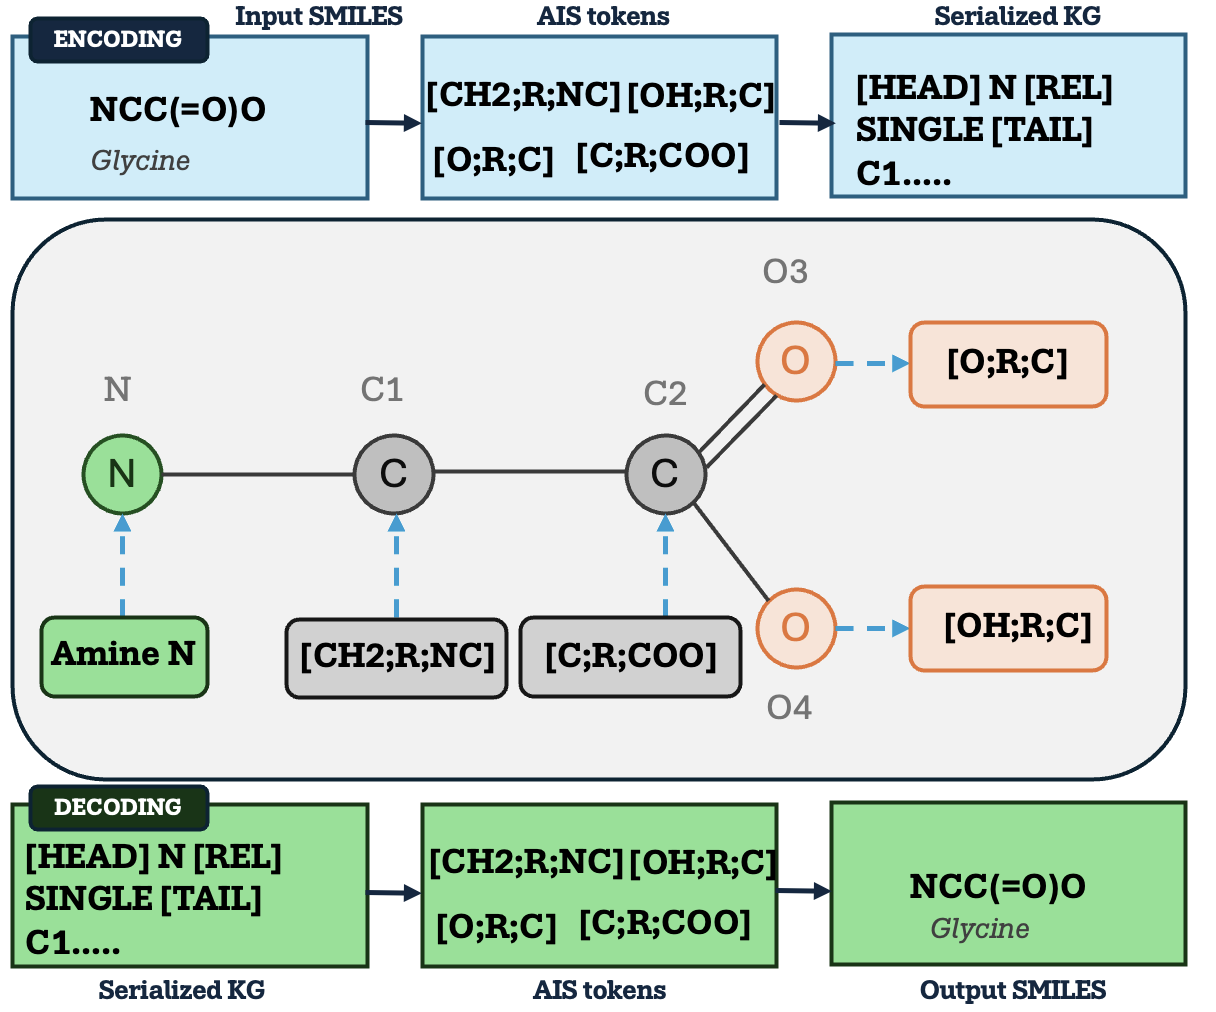
\includegraphics[width=\linewidth]{latex/Images/enc_dec.png}
    \caption{Molecule encoding and decoding in \texttt{BiMol-Diff}.}
    \label{fig:enc_dec}
    \vspace{-3mm}
\end{figure}


\noindent \textbf{Conditional Diffusion.}
For either direction, we embed the target \(\mathcal{A}\) into continuous ``clean'' latents \(\mathbf{z}_0=g_{\Phi}(\mathcal{A})\) and apply a conditional DDPM to obtain \(\mathbf{z}_t\). The reverse processes denoise conditioned on the source modality:
\(\mathcal{M}_\theta(\mathbf{z}_t,t,\tilde{\mathcal{G}})\) for G2S and
\(\mathcal{M}_\phi(\mathbf{z}_t,t,\mathbf{S_{text}})\) for S2G, enabling a unified objective across both directions.

\noindent \textbf{Token-aware Noising.}
Unlike standard data-agnostic schedules that corrupt all tokens uniformly, \texttt{BiMol-Diff} uses a token-aware, token-dependent noising strategy that preserves chemically salient tokens more conservatively. We detail the construction and use of this schedule in Sec~\ref{graph schedule}. This improves
recoverability in both directions while keeping the same diffusion
formulation across the unified framework.





%%%%%%%%%%%%%%%%%%%%%%%%%%%%%%%%%






%%%%%%%%%%%%%%%%%%%%%%%%%%%%%%%%%%%




\subsection{Graph Encoding for \texttt{BiMol-Diff}}\label{sec:graph-encoding}
In Section~\ref{sec:problem}, a molecular graph is a set of
relational triplets
\(\tilde{\mathcal{G}} = \{(h_i, r_{ij}, t_j)\}\). To integrate with transformer based encoder-decoder backbone, we
serialize this set of triplets into a single token sequence. Following the
PLM-based G2S convention, each triplet is mapped to a short template
\(\langle \texttt{[HEAD]}~h_i~\texttt{[REL]}~r_{ij}~\texttt{[TAIL]}~t_j \rangle\),
and all such segments are concatenated with a separator token \texttt{[SEP]}:
\begin{equation}
    \resizebox{0.48\textwidth}{!}{$
\begin{aligned}
\tilde{\mathcal{G}} ={}&
\langle\texttt{[HEAD]}~h_{i_1}~\texttt{[REL]}~r_{i_1 j_1}~
\texttt{[TAIL]}~t_{j_1}\rangle~\texttt{[SEP]}~\\\cdots~\texttt{[SEP]}
&\langle\texttt{[HEAD]}~h_{i_M}~\texttt{[REL]}~r_{i_M j_M}~
\texttt{[TAIL]}~t_{j_M}\rangle
\end{aligned}
$}
\end{equation}


\noindent where \(\{(i_m,j_m)\}_{m=1}^M\) enumerates all bonds with \(i_m < j_m\) to avoid
duplicates. This linearized sequence \(\tilde{\mathcal{G}}\) serves
as the conditioning signal to \texttt{BiMol-Diff} in the graph-to-sequence task. Figure~\ref{fig:enc_dec} (top) illustrates this
encoding process.

\noindent \textbf{Example (molecule KG $\rightarrow$ caption).}
Consider the molecule with SMILES string \texttt{CCO} (ethanol). Its molecular
graph has three atoms
$h_1 = \texttt{C}_1$, $h_2 = \texttt{C}_2$, $h_3 = \texttt{O}_3$
and two single bonds: $(1,2)$ and $(2,3)$. The corresponding KG triplets are
$(\texttt{C}_1,\ \texttt{SINGLE},\ \texttt{C}_2)$ and
$(\texttt{C}_2,\ \texttt{SINGLE},\ \texttt{O}_3)$.
Our serialized KG becomes
\[
\resizebox{0.48\textwidth}{!}{$
\begin{aligned}
\tilde{\mathcal{G}} =\;&
\langle \texttt{[HEAD]}~\texttt{C}_1~\texttt{[REL]}~\texttt{SINGLE}~
\texttt{[TAIL]}~\texttt{C}_2 \rangle~\texttt{[SEP]} \\
&\langle \texttt{[HEAD]}~\texttt{C}_2~\texttt{[REL]}~\texttt{SINGLE}~
\texttt{[TAIL]}~\texttt{O}_3 \rangle
\end{aligned}
$}
\]

\noindent In the G2S setting,
\texttt{BiMol-Diff} takes the graph-triplet representation $\tilde{G}$ as input
and generates a natural-language caption $\mathbf{S_{text}}$ describing the
molecule. The reverse realization path used in the S2G direction is
described separately in Section~3.4.


\subsection{Graph Decoding for \texttt{BiMol-Diff}}
In the S2G direction, conditioned on \(\mathbf{S_{text}}\), \texttt{BiMol-Diff}
predicts the serialized molecular graph sequence \(\tilde{G}\). We decode
this sequence by first parsing it into atom-bond-atom triplets
\((h_i, r_{ij}, t_j)\), and then merging these triplets to recover the
corresponding molecular graph. The recovered graph is subsequently mapped
to its AIS token representation \(G\) and canonicalized into a standard
SMILES string for S2G evaluation. Figure~\ref{fig:enc_dec} (bottom)
illustrates this decoding path.


\noindent \textbf{Example (caption $\rightarrow$ molecule KG).}
Consider the textual description corresponding to ethanol. In the S2G
direction, \texttt{BiMol-Diff} predicts the serialized graph sequence:
\begin{equation}
    \tilde{G}
=
\begin{aligned}
&\langle \texttt{[HEAD]}~\texttt{C}_1~\texttt{[REL]}~\texttt{SINGLE}~\texttt{[TAIL]}~\texttt{C}_2 \rangle~\texttt{[SEP]}\\
&\langle \texttt{[HEAD]}~\texttt{C}_2~\texttt{[REL]}~\texttt{SINGLE}~\texttt{[TAIL]}~\texttt{O}_3 \rangle .
\end{aligned}
\end{equation}
These triplets are merged to recover the molecular graph with atoms
\(C_1,C_2,O_3\) and bonds \((1,2)\) and \((2,3)\). The recovered graph
is then mapped to its molecule-side representation and canonicalized into
the SMILES string \texttt{CCO}.

\subsection{Token Aware Noising}
\label{adaptive noise}
\noindent \textbf{Motivation \& Rationale:}\label{motivation}
Standard diffusion models rely on fixed, data-agnostic noising schedules that
apply noise uniformly across all tokens. \\
We argue this is suboptimal for molecular tasks because chemically salient tokens (e.g., functional groups, stereochemistry) typically carry higher information density than structurally redundant or low-information tokens.

\noindent Under uniform noising, chemically salient tokens and
simple syntactic tokens are corrupted at the same rate, which can weaken molecular fidelity. To address this, we introduce a \emph{Token-aware noise
schedule}. We hypothesize that the model’s per-timestep
reconstruction loss $\ell_t^i$ can serve as a useful proxy for token difficulty and importance. By learning a
mapping from $\ell_t^i$ to the corresponding token's noise schedule, we preserve high information tokens while allowing information-redundant tokens to tolerate higher noise levels. This re-parametrizes the denoising path, aiming to improve generation quality in both G2S and S2G tasks.

\noindent \textbf{Noising Schedule}\label{graph schedule}:
Following the rationale discussed in Section~\ref{motivation}, for the G2S setting, we propose a token-dependent noising schedule, parameterized by a vector $\bar{\alpha}_{t, \text{new}}^i \in \mathbb{R}^N$, unlike the uniform noising with baseline cumulative schedule $\bar{\alpha}_t$ (for e.g.: \textit{sqrt}) used by standard diffusion models. This formulation has two stages summarized in Algo~\ref{alg:graph_aware_training}.

\noindent \textbf{Stage 1: Estimating token-wise difficulty.}
For each token $i$ and diffusion step $t=1,\dots,T$, we
define the denoising difficulty as:
\begin{equation}
\label{eq:loss}
\resizebox{0.85\linewidth}{!}{$
    \ell_t^{\,i}
    =
    \mathbb{E}_{\mathbf{z}_t \sim q(\mathbf{z}_t \mid \mathbf{z}_0)}
    \big\|
    \mathcal{M}_\theta(\mathbf{z}_t, t, \tilde{\mathcal{G}})^{(i)}
    - \mathbf{z}_0^{(i)}
    \big\|^2
$}
\end{equation}
Averaging over the training set yields a difficulty profile
$(\ell_1^{\,i},\dots,\ell_T^{\,i})$ for each $i$. Empirically,
$\ell_t^{\,i}$ tends to increase with $t$ (later steps are noisier), but the estimated profile is not strictly monotone. We also compute $\ell_{\min}^{\,i}=\min_t \ell_t^{\,i}$ and $\ell_{\max}^{\,i}=\max_t \ell_t^{\,i}$ to define the difficulty range for token $i$.
In Stage~2 these profiles and their ranges are used to construct a token-wise cumulative schedule, and to obtain a monotonic difficulty profile for each token $i$.

\noindent\textbf{Stage 2: Token-aware schedule.}
Given $(\ell_t^{\,i})_{t=1}^T$ and the baseline cumulative schedule
$(\bar{\alpha}_t)_{t=1}^T$, we construct an adaptive schedule
$(\bar{\alpha}_{t,\mathrm{new}}^{\,i})_{t=1}^T$ for each token $i$. Since this schedule controls noise applied at each step, we want to reallocate noise according to denoising difficulty. Hence, we define a
piecewise-linear map $\Psi_i:[\ell_{\min}^{\,i},\ell_{\max}^{\,i}]\to(0,1)$
that interpolates the baseline schedule as a function of loss:

\begin{equation}
\label{eq:mapping}
\Psi_i(x)
=
\bar{\alpha}_{t-1}
+
\frac{\bar{\alpha}_t - \bar{\alpha}_{t-1}}{\ell_t^{\,i} - \ell_{t-1}^{\,i}}\,
\big(x - \ell_{t-1}^{\,i}\big),
\end{equation}
with $x \in [\ell_{t-1}^{\,i},\, \ell_t^{\,i}),\;\; t=2,\dots,T,$    $\Psi_i(\ell_1^{\,i})=\bar{\alpha}_1$ and $\Psi_i(\ell_T^{\,i})=\bar{\alpha}_T$. In case $\ell_t^{\,i}=\ell_{t-1}^{\,i}$, we add a tiny jitter $\varepsilon$ to avoid division by zero. 
Empirically, $(\ell_t^{\,i})_{t=1}^T$ is not
strictly monotone in $t$, so instead of using its raw values we introduce a new linear ramp in difficulty space:
\begin{equation}
\label{eq:ell_ramp}
\ell_{t}^{\,i,\mathrm{new}}
=
\ell_{\min}^{\,i}
+
\frac{t-1}{T-1}\,\big(\ell_{\max}^{\,i} - \ell_{\min}^{\,i}\big)
\end{equation}
with $t=1,\dots,T$. Substituting this $\ell_{t}^{\,i,\mathrm{new}}$ into $\Psi_i(x)$ we get a new cumulative schedule 
$\bar{\alpha}_{t, \text{new}}^{\,i} = \Psi_i\!\big(\ell_{t}^{\,i,\mathrm{new}}\big)$ for $t=1,\dots,T$. 
We clamp $\bar{\alpha}_{t, \text{new}}^{\,i}$ to $(0,1)$ and apply a non-increasing isotonic projection (refer Appendix~\ref{projection}) over $t$ to obtain the final schedule 
$0 < \bar{\alpha}_{t+1,\mathrm{new}}^{\,i} \le \bar{\alpha}_{t,\mathrm{new}}^{\,i} < 1$ for all $t$. 




%%%%%%%%%%%%%%%%%%%%%%%%%%%%%%

\begin{algorithm}[t!]
\caption{Token Aware Noise Schedule}
\label{alg:graph_aware_training}
\begin{algorithmic}[1]
\REQUIRE Baseline cumulative schedule $\{\bar{\alpha}_t\}_{t=1}^T$, update interval \texttt{K}
\ENSURE Schedules $\{\bar{\alpha}^{\,i}_{t,\mathrm{new}}\}_{t=1}^T$ for all $i$

\IF{\texttt{train\_step} \% \texttt{K} $== 0$}
  \FOR{\text{all} $i$}
    \STATE Estimate $\{\ell_t^{\,i}\}_{t=1}^T$ via Eq.~\ref{eq:loss}; 
           compute $\{\ell_{\min}^{\,i}, \ell_{\max}^{\,i}\}$.
    \STATE Define piecewise-linear map $\Psi_i$ as in Eq.~(\ref{eq:mapping}).
    \STATE Construct difficulty ramp $\{\ell_{t}^{\,i,\mathrm{new}}\}_{t=1}^T$ via Eq.~(\ref{eq:ell_ramp}).
    \STATE Compute new schedule $\tilde{\alpha}_t^{\,i} = \Psi_i(\ell_{t}^{\,i,\mathrm{new}})$.
    \STATE Clamp $\tilde{\alpha}_t^{\,i}$ to $(0,1)$, apply a non-increasing
           isotonic projection to obtain 
           $\{\bar{\alpha}^{\,i}_{t,\mathrm{new}}\}_{t=1}^T$.
  \ENDFOR
\ENDIF

\RETURN $\{\bar{\alpha}^{\,i}_{t,\mathrm{new}}\}$ for all tokens $i$ and steps $t$.
\end{algorithmic}
\end{algorithm}
\vspace{-4mm}

\subsection{Model Training and Inference}
\begin{table*}[t!]
    \centering
    \tiny
    \resizebox{0.8\textwidth}{!}{%
    \begin{tabular}{l c c c c c c}
        \toprule
        \textbf{Method} & \textbf{\#P} & \textbf{B} & \textbf{CrF++} & \textbf{M} & \textbf{B-F1} & \textbf{MVE} \\
        \midrule
        
        % --- Group 1: Autoregressive Baselines ---
        \multicolumn{7}{l}{\textbf{Autoregressive Baselines}} \\
        MolT5-Base~\citep{edwards-etal-2022-translation} & 220M & 0.452 & 0.651 & 0.510 & 0.681 & 0.852 \\
        Text+Chem T5~\citep{christofidellis2023textchemt5} & 223M & \underline{0.542} & \underline{0.701} & 0.648 & 0.728 & 0.866 \\
        MolCA~\citep{liu2024molcamoleculargraphlanguagemodeling} & 110M & 0.531 & 0.665 & \textbf{0.651} & 0.709 & 0.815 \\
        GitMol~\citep{Liu_2024} & 700M & 0.475 & 0.680 & 0.532 & 0.751 & 0.875 \\
        GraphT5~\citep{kim2025grapht5unifiedmoleculargraphlanguage} & 272M & 0.481 & 0.692 & 0.545 & \underline{0.810} & \underline{0.913} \\

        \midrule
        
        % --- Group 2: Diffusion Baselines ---
        \multicolumn{7}{l}{\textbf{Diffusion Baselines}} \\
        Diffusion-LM~\citep{li2022diffusionlmimprovescontrollabletext} & 91M & 0.512 & 0.702 & 0.602 & 0.783 & 0.861 \\
        DiffuSeq~\citep{gong2023diffuseqsequencesequencetext} & 91M & 0.532 & 0.708 & 0.601 & 0.812 & 0.887 \\
        TGM-DLM~\citep{gong2024tgmdlm} & 125M & 0.467 & 0.689 & 0.589 & 0.779 & 0.856 \\

        \midrule
        
        % --- Group 3: Ours ---
        \rowcolor{white!70!yellow}
        % \texttt{BiMol-Diff}-1.0 (ours) & 50M & 0.534 & 0.715 & 0.560 & 0.816 & 0.901 \\
        \rowcolor{white!70!yellow}
        \texttt{BiMol-Diff} (ours) & 63M & \textbf{0.567} & \textbf{0.734} & 0.626 & \textbf{0.843} & \textbf{0.925} \\

        % Gain Rows: Comparing against best in respective categories
        \rowcolor{white!70!gray}
        \%Gain (vs. Best AR) & \textbf{x3.5$\downarrow$} & \textbf{+4.6\%} & \textbf{+4.7\%} & -3.8\% & \textbf{+4.1\%} & \textbf{+1.3\%} \\
        \rowcolor{white!70!gray}
        \%Gain (vs. Best Diff) & \textbf{x1.4$\downarrow$} & \textbf{+6.6\%} & \textbf{+3.7\%} & \textbf{+4.2\%} & \textbf{+3.8\%} & \textbf{+4.3\%} \\
        \bottomrule
    \end{tabular}%
    }
    \caption{Molecule captioning performance on the M3-20M dataset. Benchmarking \texttt{BiMol-Diff} against SoTA Autoregressive (AR) and Diffusion models. \texttt{BiMol-Diff} achieves state-of-the-art results, surpassing the best diffusion and AR baselines by substantial margins across all metrics while using fewer parameters.}
    \label{molecule captioning}
    \vspace{-3mm}
\end{table*}



\noindent \textbf{Training}: Our training objective is derived from the Variational Lower Bound (VLB) (Eq. 2) presented in the preliminaries. While the full VLB optimization can be unstable \citep{ho2020denoisingdiffusionprobabilisticmodels}, 
a common simplification is to train the model $\mathcal{M}_\theta$ to predict the added noise $\boldsymbol{\epsilon}$. However, our framework adopts an alternative $\mathbf{z}_0$-prediction reparameterization, which trains the model to directly predict the clean data $\mathbf{z}_0$ at every timestep $t$.
A critical component of this objective is the rounding term $L_0 = -\log \tilde{p}_\Phi(\mathbf{S_{text}} \mid \mathbf{z}_0)$, which handles the final step of converting the continuous latent variable $\mathbf{z}_0$ back into discrete tokens $\mathbf{S_{text}}$. We define this as a trainable rounding distribution: $\tilde{p}_\Phi(\mathbf{S_{text}} \mid \mathbf{z}_0) = \prod_{i=1}^{N} \tilde{p}_\Phi(s_i \mid \mathbf{z}_{0,i})$,
where each token $s_i$ is sampled from a softmax distribution over the vocabulary, using logits derived from the corresponding output embedding $\mathbf{z}_{0,i}$.
By combining this rounding term (for $t=0$) with the denoising matching terms (for $t>1$) using our $\mathbf{z}_0$-prediction reparameterization, we arrive at our final, composite objective. (The full derivation from the VLB is in App \ref{sec:derivation_appendix}).

\begin{equation}
\label{z0-pred}
\resizebox{0.85\columnwidth}{!}{
$
\begin{aligned}
\mathcal{L}_{\text{e2e-simple}}(\mathbf{S_{text}}) = \mathbb{E}_{q} 
    \Bigl[ \sum_{t=2}^{T} \underbrace{\|\mathcal{M}_\theta(\mathbf{z}_t, t, \tilde{\mathcal{G}}) - \mathbf{z}_0 \|^2}_{\text{Denoising}} + \\\underbrace{\|\,g_\Phi(\mathbf{S_{text}}) - \mathcal{M}_\theta(\mathbf{z}_1, 1, \tilde{\mathcal{G}})\|^2}_{\text{Consistency}} - \underbrace{\log \tilde{p}_\Phi(\mathbf{S_{text}} \mid \mathbf{z}_0)}_{\text{Rounding}} \Bigr]
\end{aligned}
$
}
\end{equation}
The same objective is used in the S2G direction, with the target discrete sequence replaced by \(\tilde{G}\) and the conditioning sequence replaced by \(S_{\text{text}}\).
This objective directly optimizes the most critical parts of the process: the denoising accuracy across all steps (Denoising), the consistency of the first denoising step with the true data embedding (Consistency), and the quality of the final conversion to discrete tokens (Rounding)\label{rounding}. 

\noindent \textbf{Inference-time schedule:}
The $\mathbf{z}_0$-prediction objective (Eq:~\ref{z0-pred}) trains the denoiser to explicitly predict the clean latent at each step.
At inference, given $\mathbf{z}_t$ and conditioning context $\mathbf{c}$, we compute
$\hat{\mathbf{z}}_0 = \mathcal{M}_\theta(\mathbf{z}_t, t, \mathbf{c})$
(with $\mathbf{c}=\tilde{\mathcal{G}}$ for G2S and $\mathbf{c}=\mathbf{S_{text}}$ for S2G).
We then use our learned token-wise cumulative schedule $\bar{\alpha}^{\,i}_{t,\mathrm{new}}$ in the reverse sampling update, where $\boldsymbol{\epsilon}\sim\mathcal{N}(\mathbf{0},\mathbf{I})$.
To mitigate rounding errors (refer section~\ref{rounding}), we apply the clamping trick, which forces the predicted vector to commit to a word for intermediate diffusion steps:
\begin{equation}
\label{eq:inference_schedule}
\resizebox{0.85\columnwidth}{!}{$
\begin{aligned}
\mathbf{z}^{(i)}_{t-1}
&=
\sqrt{\bar{\alpha}^{\,i}_{t-1,\mathrm{new}}}\;\mathrm{Clamp}\!\Big(\mathcal{M}_\theta(\mathbf{z}_t, t, \mathbf{c})^{(i)}\Big) \\
&\quad+\;
\sqrt{1-\bar{\alpha}^{\,i}_{t-1,\mathrm{new}}}\;\boldsymbol{\epsilon}^{(i)},
\end{aligned}
$}
\end{equation}
\noindent where $\mathrm{Clamp}(\cdot)$ denotes nearest-neighbor projection onto the embedding table.
This strategy ensures that the diffusion trajectory remains grounded in valid token embeddings during sampling.

\begin{table*}[t!]
    \centering
    \tiny
    \resizebox{0.8\textwidth}{!}{%
    \begin{tabular}{l c c c c c c c}
        \toprule
        \textbf{Method} & \textbf{Type} & \textbf{\#P} & \textbf{Exact} & \textbf{MACCS} & \textbf{RDK} & \textbf{Morgan} & \textbf{Valid} \\
        \midrule
        % --- Group 1: Text AR (SMILES) ---
        \multicolumn{8}{l}{\textbf{Text-Based Autoregressive (SMILES)}} \\
        T5-Base~\citep{JMLR:v21:20-074} & AR & 248M & 0.069 & 0.731 & 0.605 & 0.545 & 0.660 \\
        MolT5-Base~\citep{edwards-etal-2022-translation} & AR & 248M & 0.081 & 0.721 & 0.588 & 0.529 & 0.772 \\
        MolXPT~\citep{liu-etal-2023-molxpt} & AR & 350M & 0.215 & \textbf{0.859} & \textbf{0.757} & \textbf{0.667} & \textbf{0.983} \\
        T5 Enc + MolXPT MLP~\citep{Deng_2025} & Adapter & 111M & \textbf{0.227} & 0.820 & 0.713 & 0.636 & 0.980 \\
        %
        \midrule
        % --- Group 2: Text AR (SELFIES) ---
        \multicolumn{8}{l}{\textbf{Text-Based Autoregressive (SELFIES)}} \\
        SciBERT + MolGen~\citep{Deng_2025} & Adapter & 317M & 0.083 & 0.680 & 0.526 & 0.422 & 0.995 \\
        Galactica-1.3B + MolGen~\citep{fang2024domainagnosticmoleculargenerationchemical} & Adapter & 1.5B & 0.091 & 0.706 & 0.560 & 0.454 & \underline{0.995} \\
        T5 Enc + MolGen~\citep{Deng_2025} & Adapter & 317M & 0.165 & 0.758 & 0.616 & 0.527 & 0.995 \\
        %
        \midrule
        % --- Group 3: Graph / Diffusion Baselines ---
        \multicolumn{8}{l}{\textbf{Graph \& Diffusion Baselines}} \\
        DiGress (sim. guidance)~\citep{vignac2023digressdiscretedenoisingdiffusion} & Diff & 289M & 0.014 & 0.577 & 0.389 & 0.288 & 0.854 \\
        3M-Diffusion~\citep{zhu20243mdiffusionlatentmultimodaldiffusion} & Diff & 162M & 0.005 & 0.548 & 0.370 & 0.273 & \textbf{1.000} \\
        Graph-DiT~\citep{liu2024graphdit} & Diff & 162M & 0.000 & 0.374 & 0.269 & 0.159 & 0.909 \\
        UTGDiff (w/o pretrain)~\citep{xiang2025instructionbasedmoleculargraphgeneration} & Diff & 125M & \underline{0.227} & \underline{0.867} & \underline{0.763} & \underline{0.695} & 0.856 \\
        %
        \midrule
        
        \rowcolor{white!70!yellow}
        \texttt{BiMol-Diff} (ours) & Diff & 180M & \textbf{0.262} & \textbf{0.894} & \textbf{0.791} & \textbf{0.762} & 0.901 \\
        
        \rowcolor{white!70!gray}
        \%Gain (vs. Best AR) & -- & \textbf{x1.9$\downarrow$} & \textbf{+15.4\%} & \textbf{+4.1\%} & \textbf{+4.5\%} & \textbf{+14.2\%} & -8.3\% \\
        
       
        \rowcolor{white!70!gray}
        \%Gain (vs. Best Diff) & -- & \textbf{x1$\downarrow$} & \textbf{+15.4\%} & \textbf{+3.1\%} & \textbf{+3.7\%} & \textbf{+9.6\%} & \textbf{+5.3\%} \\
        \bottomrule
    \end{tabular}%
    }
    \caption{Molecule generation performance on the ChEBI-20 test set. \texttt{BiMol-Diff} outperforms state-of-the-art Autoregressive and Diffusion baselines in structure reconstruction (Exact Match) and fingerprint similarity, validating the effectiveness of token-aware denoising.}
    \label{molecule generation}
    \vspace{-4mm}
\end{table*}

